% Options for packages loaded elsewhere
\PassOptionsToPackage{unicode}{hyperref}
\PassOptionsToPackage{hyphens}{url}
\PassOptionsToPackage{dvipsnames,svgnames,x11names}{xcolor}
%
\documentclass[
  letterpaper,
  DIV=11,
  numbers=noendperiod]{scrartcl}

\usepackage{amsmath,amssymb}
\usepackage{iftex}
\ifPDFTeX
  \usepackage[T1]{fontenc}
  \usepackage[utf8]{inputenc}
  \usepackage{textcomp} % provide euro and other symbols
\else % if luatex or xetex
  \usepackage{unicode-math}
  \defaultfontfeatures{Scale=MatchLowercase}
  \defaultfontfeatures[\rmfamily]{Ligatures=TeX,Scale=1}
\fi
\usepackage{lmodern}
\ifPDFTeX\else  
    % xetex/luatex font selection
\fi
% Use upquote if available, for straight quotes in verbatim environments
\IfFileExists{upquote.sty}{\usepackage{upquote}}{}
\IfFileExists{microtype.sty}{% use microtype if available
  \usepackage[]{microtype}
  \UseMicrotypeSet[protrusion]{basicmath} % disable protrusion for tt fonts
}{}
\makeatletter
\@ifundefined{KOMAClassName}{% if non-KOMA class
  \IfFileExists{parskip.sty}{%
    \usepackage{parskip}
  }{% else
    \setlength{\parindent}{0pt}
    \setlength{\parskip}{6pt plus 2pt minus 1pt}}
}{% if KOMA class
  \KOMAoptions{parskip=half}}
\makeatother
\usepackage{xcolor}
\setlength{\emergencystretch}{3em} % prevent overfull lines
\setcounter{secnumdepth}{5}
% Make \paragraph and \subparagraph free-standing
\makeatletter
\ifx\paragraph\undefined\else
  \let\oldparagraph\paragraph
  \renewcommand{\paragraph}{
    \@ifstar
      \xxxParagraphStar
      \xxxParagraphNoStar
  }
  \newcommand{\xxxParagraphStar}[1]{\oldparagraph*{#1}\mbox{}}
  \newcommand{\xxxParagraphNoStar}[1]{\oldparagraph{#1}\mbox{}}
\fi
\ifx\subparagraph\undefined\else
  \let\oldsubparagraph\subparagraph
  \renewcommand{\subparagraph}{
    \@ifstar
      \xxxSubParagraphStar
      \xxxSubParagraphNoStar
  }
  \newcommand{\xxxSubParagraphStar}[1]{\oldsubparagraph*{#1}\mbox{}}
  \newcommand{\xxxSubParagraphNoStar}[1]{\oldsubparagraph{#1}\mbox{}}
\fi
\makeatother

\usepackage{color}
\usepackage{fancyvrb}
\newcommand{\VerbBar}{|}
\newcommand{\VERB}{\Verb[commandchars=\\\{\}]}
\DefineVerbatimEnvironment{Highlighting}{Verbatim}{commandchars=\\\{\}}
% Add ',fontsize=\small' for more characters per line
\usepackage{framed}
\definecolor{shadecolor}{RGB}{241,243,245}
\newenvironment{Shaded}{\begin{snugshade}}{\end{snugshade}}
\newcommand{\AlertTok}[1]{\textcolor[rgb]{0.68,0.00,0.00}{#1}}
\newcommand{\AnnotationTok}[1]{\textcolor[rgb]{0.37,0.37,0.37}{#1}}
\newcommand{\AttributeTok}[1]{\textcolor[rgb]{0.40,0.45,0.13}{#1}}
\newcommand{\BaseNTok}[1]{\textcolor[rgb]{0.68,0.00,0.00}{#1}}
\newcommand{\BuiltInTok}[1]{\textcolor[rgb]{0.00,0.23,0.31}{#1}}
\newcommand{\CharTok}[1]{\textcolor[rgb]{0.13,0.47,0.30}{#1}}
\newcommand{\CommentTok}[1]{\textcolor[rgb]{0.37,0.37,0.37}{#1}}
\newcommand{\CommentVarTok}[1]{\textcolor[rgb]{0.37,0.37,0.37}{\textit{#1}}}
\newcommand{\ConstantTok}[1]{\textcolor[rgb]{0.56,0.35,0.01}{#1}}
\newcommand{\ControlFlowTok}[1]{\textcolor[rgb]{0.00,0.23,0.31}{\textbf{#1}}}
\newcommand{\DataTypeTok}[1]{\textcolor[rgb]{0.68,0.00,0.00}{#1}}
\newcommand{\DecValTok}[1]{\textcolor[rgb]{0.68,0.00,0.00}{#1}}
\newcommand{\DocumentationTok}[1]{\textcolor[rgb]{0.37,0.37,0.37}{\textit{#1}}}
\newcommand{\ErrorTok}[1]{\textcolor[rgb]{0.68,0.00,0.00}{#1}}
\newcommand{\ExtensionTok}[1]{\textcolor[rgb]{0.00,0.23,0.31}{#1}}
\newcommand{\FloatTok}[1]{\textcolor[rgb]{0.68,0.00,0.00}{#1}}
\newcommand{\FunctionTok}[1]{\textcolor[rgb]{0.28,0.35,0.67}{#1}}
\newcommand{\ImportTok}[1]{\textcolor[rgb]{0.00,0.46,0.62}{#1}}
\newcommand{\InformationTok}[1]{\textcolor[rgb]{0.37,0.37,0.37}{#1}}
\newcommand{\KeywordTok}[1]{\textcolor[rgb]{0.00,0.23,0.31}{\textbf{#1}}}
\newcommand{\NormalTok}[1]{\textcolor[rgb]{0.00,0.23,0.31}{#1}}
\newcommand{\OperatorTok}[1]{\textcolor[rgb]{0.37,0.37,0.37}{#1}}
\newcommand{\OtherTok}[1]{\textcolor[rgb]{0.00,0.23,0.31}{#1}}
\newcommand{\PreprocessorTok}[1]{\textcolor[rgb]{0.68,0.00,0.00}{#1}}
\newcommand{\RegionMarkerTok}[1]{\textcolor[rgb]{0.00,0.23,0.31}{#1}}
\newcommand{\SpecialCharTok}[1]{\textcolor[rgb]{0.37,0.37,0.37}{#1}}
\newcommand{\SpecialStringTok}[1]{\textcolor[rgb]{0.13,0.47,0.30}{#1}}
\newcommand{\StringTok}[1]{\textcolor[rgb]{0.13,0.47,0.30}{#1}}
\newcommand{\VariableTok}[1]{\textcolor[rgb]{0.07,0.07,0.07}{#1}}
\newcommand{\VerbatimStringTok}[1]{\textcolor[rgb]{0.13,0.47,0.30}{#1}}
\newcommand{\WarningTok}[1]{\textcolor[rgb]{0.37,0.37,0.37}{\textit{#1}}}

\providecommand{\tightlist}{%
  \setlength{\itemsep}{0pt}\setlength{\parskip}{0pt}}\usepackage{longtable,booktabs,array}
\usepackage{calc} % for calculating minipage widths
% Correct order of tables after \paragraph or \subparagraph
\usepackage{etoolbox}
\makeatletter
\patchcmd\longtable{\par}{\if@noskipsec\mbox{}\fi\par}{}{}
\makeatother
% Allow footnotes in longtable head/foot
\IfFileExists{footnotehyper.sty}{\usepackage{footnotehyper}}{\usepackage{footnote}}
\makesavenoteenv{longtable}
\usepackage{graphicx}
\makeatletter
\def\maxwidth{\ifdim\Gin@nat@width>\linewidth\linewidth\else\Gin@nat@width\fi}
\def\maxheight{\ifdim\Gin@nat@height>\textheight\textheight\else\Gin@nat@height\fi}
\makeatother
% Scale images if necessary, so that they will not overflow the page
% margins by default, and it is still possible to overwrite the defaults
% using explicit options in \includegraphics[width, height, ...]{}
\setkeys{Gin}{width=\maxwidth,height=\maxheight,keepaspectratio}
% Set default figure placement to htbp
\makeatletter
\def\fps@figure{htbp}
\makeatother

\KOMAoption{captions}{tableheading,figureheading}
\makeatletter
\@ifpackageloaded{caption}{}{\usepackage{caption}}
\AtBeginDocument{%
\ifdefined\contentsname
  \renewcommand*\contentsname{Table of contents}
\else
  \newcommand\contentsname{Table of contents}
\fi
\ifdefined\listfigurename
  \renewcommand*\listfigurename{List of Figures}
\else
  \newcommand\listfigurename{List of Figures}
\fi
\ifdefined\listtablename
  \renewcommand*\listtablename{List of Tables}
\else
  \newcommand\listtablename{List of Tables}
\fi
\ifdefined\figurename
  \renewcommand*\figurename{Figure}
\else
  \newcommand\figurename{Figure}
\fi
\ifdefined\tablename
  \renewcommand*\tablename{Table}
\else
  \newcommand\tablename{Table}
\fi
}
\@ifpackageloaded{float}{}{\usepackage{float}}
\floatstyle{ruled}
\@ifundefined{c@chapter}{\newfloat{codelisting}{h}{lop}}{\newfloat{codelisting}{h}{lop}[chapter]}
\floatname{codelisting}{Listing}
\newcommand*\listoflistings{\listof{codelisting}{List of Listings}}
\makeatother
\makeatletter
\makeatother
\makeatletter
\@ifpackageloaded{caption}{}{\usepackage{caption}}
\@ifpackageloaded{subcaption}{}{\usepackage{subcaption}}
\makeatother

\ifLuaTeX
  \usepackage{selnolig}  % disable illegal ligatures
\fi
\usepackage{bookmark}

\IfFileExists{xurl.sty}{\usepackage{xurl}}{} % add URL line breaks if available
\urlstyle{same} % disable monospaced font for URLs
\hypersetup{
  pdftitle={STA107 Post-Course Survey Analysis},
  pdfauthor={Sinan Ma; Jaiditya Dev},
  colorlinks=true,
  linkcolor={blue},
  filecolor={Maroon},
  citecolor={Blue},
  urlcolor={Blue},
  pdfcreator={LaTeX via pandoc}}


\title{STA107 Post-Course Survey Analysis}
\usepackage{etoolbox}
\makeatletter
\providecommand{\subtitle}[1]{% add subtitle to \maketitle
  \apptocmd{\@title}{\par {\large #1 \par}}{}{}
}
\makeatother
\subtitle{Evaluating Student Reflections on R and Statistical Learning}
\author{Sinan Ma \and Jaiditya Dev}
\date{2025-04-13}

\begin{document}
\maketitle

\renewcommand*\contentsname{Table of contents}
{
\hypersetup{linkcolor=}
\setcounter{tocdepth}{3}
\tableofcontents
}

\section{Introduction}\label{introduction}

This report presents an analysis of the anonymous post-course survey
completed by students enrolled in \textbf{STA107: Introduction to
Statistics} at the University of Toronto Mississauga. The survey was
voluntary, open for multiple submissions, and contributed \textbf{2\% to
the course grade}. Its goal was to evaluate students' experiences with
R-based activities, the integration of normal distribution concepts, and
overall satisfaction with the course components. This feedback will help
refine future course offerings and improve the learning experience.

\section{Survey Questions}\label{survey-questions}

This section outlines the structure of the survey and highlights key
question types:

\begin{itemize}
\tightlist
\item
  \textbf{Quantitative items}: Likert-scale responses on course clarity,
  usefulness of R exercises, and understanding of statistical concepts.
\item
  \textbf{Qualitative items}: Open-ended prompts for students to share
  what they found most/least helpful and suggestions for improvement.
\end{itemize}

The post-course survey comprised 17 open- and close-ended questions.
Among these, 11 were qualitative in nature (\texttt{Q3}, \texttt{Q6},
\texttt{Q8}, \texttt{Q10}, \texttt{Q11}, \texttt{Q12}, \texttt{Q13},
\texttt{Q14}, \texttt{Q15}, \texttt{Q16}, \texttt{Q17}), focusing on
free-text responses reflecting students' thoughts on the content,
instruction, and overall experience.

\section{Data Analysis}\label{data-analysis}

\subsection{Methodology}\label{methodology}

We employed a \textbf{mixed-methods approach}:

\begin{itemize}
\tightlist
\item
  \textbf{Quantitative analysis}: Descriptive statistics and
  visualizations for Likert-scale questions.
\item
  \textbf{Qualitative analysis}: Thematic coding of open-ended responses
  to identify common sentiments and suggestions.
\end{itemize}

\subsubsection{Qualitative Analysis}\label{qualitative-analysis}

\begin{Shaded}
\begin{Highlighting}[]
\CommentTok{\# Load required libraries}
\FunctionTok{library}\NormalTok{(tidyverse)}
\FunctionTok{library}\NormalTok{(stringr)}
\FunctionTok{library}\NormalTok{(tidytext)}
\FunctionTok{library}\NormalTok{(syuzhet)}
\FunctionTok{library}\NormalTok{(ggplot2)}
\FunctionTok{library}\NormalTok{(tidyr)}
\FunctionTok{library}\NormalTok{(wordcloud)}
\end{Highlighting}
\end{Shaded}

\begin{verbatim}
Loading required package: RColorBrewer
\end{verbatim}

\begin{Shaded}
\begin{Highlighting}[]
\CommentTok{\# Read in the survey data}
\NormalTok{data }\OtherTok{\textless{}{-}}\NormalTok{ qualitative\_data}

\CommentTok{\# Rename columns}
\FunctionTok{colnames}\NormalTok{(data)[}\DecValTok{1}\SpecialCharTok{:}\DecValTok{11}\NormalTok{] }\OtherTok{\textless{}{-}} \FunctionTok{c}\NormalTok{(}\StringTok{"Q3"}\NormalTok{, }\StringTok{"Q6"}\NormalTok{, }\StringTok{"Q8"}\NormalTok{, }\StringTok{"Q10"}\NormalTok{, }\StringTok{"Q11"}\NormalTok{, }
                          \StringTok{"Q12"}\NormalTok{, }\StringTok{"Q13"}\NormalTok{, }\StringTok{"Q14"}\NormalTok{, }\StringTok{"Q15"}\NormalTok{, }\StringTok{"Q16"}\NormalTok{, }\StringTok{"Q17"}\NormalTok{)}

\CommentTok{\# Clean the text}
\NormalTok{data\_clean }\OtherTok{\textless{}{-}}\NormalTok{ data }\SpecialCharTok{\%\textgreater{}\%}
  \FunctionTok{mutate}\NormalTok{(}\FunctionTok{across}\NormalTok{(}\FunctionTok{everything}\NormalTok{(), }\SpecialCharTok{\textasciitilde{}} \FunctionTok{str\_trim}\NormalTok{(}\FunctionTok{tolower}\NormalTok{(}\FunctionTok{as.character}\NormalTok{(.)))))}

\CommentTok{\# Initialize an empty data frame to collect sentiment results}
\NormalTok{sentiment\_results }\OtherTok{\textless{}{-}} \FunctionTok{data.frame}\NormalTok{(}
  \AttributeTok{Question =} \FunctionTok{character}\NormalTok{(),}
  \AttributeTok{Positive =} \FunctionTok{numeric}\NormalTok{(),}
  \AttributeTok{Negative =} \FunctionTok{numeric}\NormalTok{(),}
  \AttributeTok{Neutral =} \FunctionTok{numeric}\NormalTok{(),}
  \AttributeTok{stringsAsFactors =} \ConstantTok{FALSE}
\NormalTok{)}

\CommentTok{\# Function to calculate sentiment}
\NormalTok{analyze\_sentiment }\OtherTok{\textless{}{-}} \ControlFlowTok{function}\NormalTok{(question\_col, question\_name) \{}
\NormalTok{  sentiments }\OtherTok{\textless{}{-}} \FunctionTok{get\_nrc\_sentiment}\NormalTok{(data\_clean[[question\_col]])}
  
\NormalTok{  pos }\OtherTok{\textless{}{-}} \FunctionTok{sum}\NormalTok{(sentiments}\SpecialCharTok{$}\NormalTok{positive)}
\NormalTok{  neg }\OtherTok{\textless{}{-}} \FunctionTok{sum}\NormalTok{(sentiments}\SpecialCharTok{$}\NormalTok{negative)}
\NormalTok{  neutral }\OtherTok{\textless{}{-}} \FunctionTok{nrow}\NormalTok{(sentiments) }\SpecialCharTok{{-}} 
    \FunctionTok{sum}\NormalTok{(}\FunctionTok{rowSums}\NormalTok{(sentiments[, }\FunctionTok{c}\NormalTok{(}\StringTok{"positive"}\NormalTok{, }\StringTok{"negative"}\NormalTok{)]) }\SpecialCharTok{\textgreater{}} \DecValTok{0}\NormalTok{)}
  
\NormalTok{  sentiment\_results }\OtherTok{\textless{}\textless{}{-}} \FunctionTok{rbind}\NormalTok{(sentiment\_results, }\FunctionTok{data.frame}\NormalTok{(}
    \AttributeTok{Question =}\NormalTok{ question\_name,}
    \AttributeTok{Positive =}\NormalTok{ pos,}
    \AttributeTok{Negative =}\NormalTok{ neg,}
    \AttributeTok{Neutral =}\NormalTok{ neutral}
\NormalTok{  ))}
\NormalTok{\}}

\CommentTok{\# Apply the function to all relevant questions}
\NormalTok{question\_names }\OtherTok{\textless{}{-}} \FunctionTok{c}\NormalTok{(}\StringTok{"Q3"}\NormalTok{, }\StringTok{"Q6"}\NormalTok{, }\StringTok{"Q8"}\NormalTok{, }\StringTok{"Q10"}\NormalTok{, }\StringTok{"Q11"}\NormalTok{, }
                    \StringTok{"Q12"}\NormalTok{, }\StringTok{"Q13"}\NormalTok{, }\StringTok{"Q14"}\NormalTok{, }\StringTok{"Q15"}\NormalTok{, }\StringTok{"Q16"}\NormalTok{, }\StringTok{"Q17"}\NormalTok{)}

\ControlFlowTok{for}\NormalTok{ (qn }\ControlFlowTok{in}\NormalTok{ question\_names) \{}
  \FunctionTok{analyze\_sentiment}\NormalTok{(qn, qn)}
\NormalTok{\}}
\end{Highlighting}
\end{Shaded}

\section{Results}\label{results}

\subsection{Quantitative Results}\label{quantitative-results}

\begin{itemize}
\tightlist
\item
  Distribution of responses to Likert-scale questions
\item
  Summary statistics (mean, median, SD)
\item
  Visualizations: bar plots, histograms
\end{itemize}

\subsection{Qualitative Results}\label{qualitative-results}

The sentiment analysis revealed a clear trend of positive student
engagement across most open-ended responses. When asked about what
aspects of the course were most helpful, students consistently expressed
appreciation for the structured content delivery, use of R, and clarity
in statistical explanations. Similarly, reflections on the usefulness of
the normal model and applied examples elicited strong positive
sentiment, highlighting the effectiveness of concept integration
throughout the term.

Feedback on the clarity of teaching and accessibility of course material
was more mixed. While many students praised the instructor's effort and
teaching style, others noted inconsistencies in understanding due to the
pace of delivery or difficulty following complex R assignments.

The most critical responses were seen in prompts asking what aspects of
the course were least helpful and what improvements could be made. Here,
students frequently cited the fast pace of certain topics, confusion
around R syntax, and a need for more real-world or scaffolded examples.
Words like ``confusing,'' ``fast,'' and ``examples'' frequently appeared
in these responses, pointing to the need for clearer instructional
supports.

\begin{figure}[H]

\caption{Sentiment Distribution by Survey Question}

{\centering 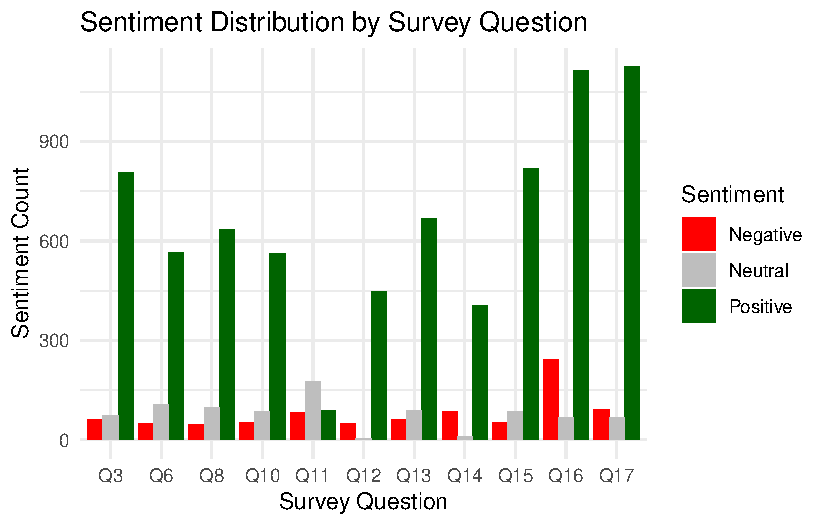
\includegraphics{paper_files/figure-pdf/sentiment-plot-1.pdf}

}

\end{figure}%

\section{Conclusion}\label{conclusion}

The STA107 post-course survey provides valuable insights into how
students perceive the course structure and its technical components.
Findings highlight both effective practices and opportunities for
enhancement. Continued evaluation and iteration will ensure the course
remains responsive to student needs and pedagogical best practices.

From a qualitative perspective, student feedback revealed strong
appreciation for several key elements of the course---especially the
hands-on R activities, the integration of real-world statistical
examples, and the clarity of normal model explanations. These components
were described as engaging and instructive, affirming their value in
helping students apply theoretical knowledge in practical settings.

However, when students were asked about areas of improvement, many
raised concerns regarding the speed at which complex topics were
introduced, as well as the difficulty of interpreting R-based
assignments without more structured guidance. Themes of pacing, clarity,
and the need for more scaffolded instruction were particularly
prominent. Addressing these concerns by slowing down the delivery of
technical material, providing more detailed examples, and incorporating
mid-semester feedback opportunities could significantly enhance the
learning experience in future offerings of STA107.

\section{References}\label{references}

\begin{itemize}
\item
  Jockers, M. (2017). \emph{syuzhet: Extracts Sentiment and
  Sentiment-Derived Plot Arcs from Text} (R package v1.0.4).
  \href{https://cran.r-project.org/web/packages/syuzhet/index.html}{CRAN
  Documentation}
\item
  Jockers, M. (2020). \emph{Introduction to the Syuzhet Package}.
  \href{https://cran.r-project.org/web/packages/syuzhet/vignettes/syuzhet-vignette.html}{CRAN
  Vignette}
\item
  Kim, H. (2022). Sentiment Analysis: Limits and Progress of the Syuzhet
  Package and Its Lexicons. \emph{Digital Humanities Quarterly, 16}(2).
  \href{http://www.digitalhumanities.org/dhq/vol/16/2/000601/000601.html}{Article}
\end{itemize}




\end{document}
